\begin{enumerate}[label=\thesection.\arabic*.,ref=\thesection.\theenumi]
\numberwithin{equation}{enumi}

\item For a unity feedback system shown in Fig. 1
\begin{align}
G(s) =\frac{K}{s(s+2)(s+4)(s+6)}
\label{eq:es17btech11019_system1}
\end{align}
Design a lag lead compensator to yield a $K_v$ = 2 and a phase margin of 30\degree.
First we will design a lead compensator and for that whole system we will design a lag compensator which will finally be the lag lead compensator of the orignal transfer function.


\solution 
For unity feedback we have Velocity error constant $\brak{K_v}$

\begin{align}
K_v &= \lim_{s \to 0} s G\brak{s} 
\label{eq:es17btech11019_Kv}
\end{align}

\begin{align}
\lim_{s \to 0} \brak{\frac{K}{\brak{2+s}\brak{4+s}\brak{6+s}} }& = 2 
\\
\implies K = 96
\label{eq:es17btech11019_init_cond}
\end{align}
Check the phase margin and gain crossover frequency by running the following code
\begin{lstlisting}
codes/es17btech11019_1.py
\end{lstlisting}
\begin{itemize}
    \item The Phase margin: $19.76\degree$
    \item Gain Crossover Frequency:1.469  rad/sec
\end{itemize}
The plot of system is as shown,
\begin{figure}[!ht]
  \centering
  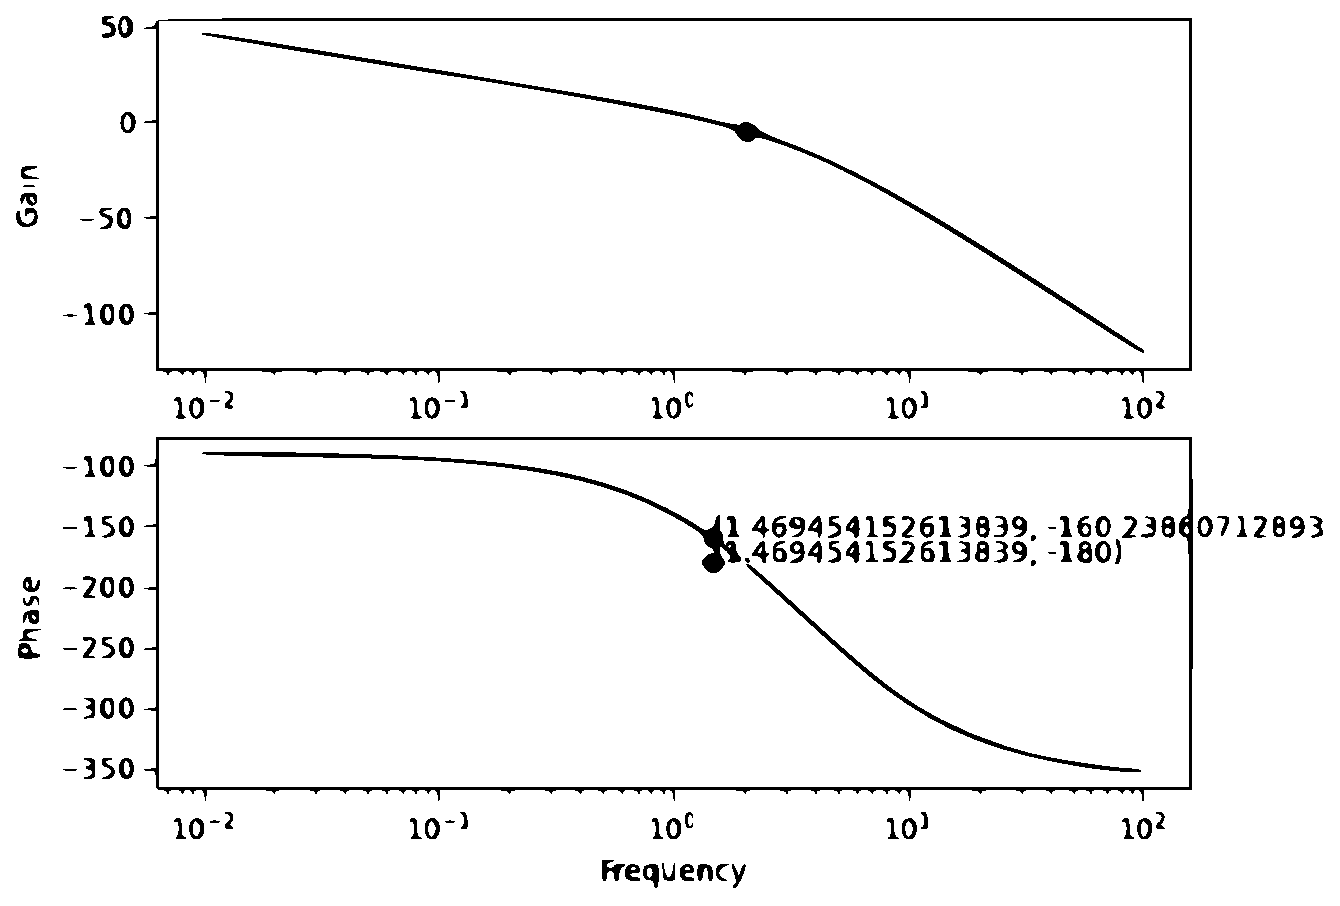
\includegraphics[width=\columnwidth]{./figs/es17btech11019_1.eps}
  \caption{}
  \label{fig:es17btech11019_1}
\end{figure}

Therefor amount of phase to be added: 30-19.76=10.24

Transfer function:
\begin{align}
C(s)=\beta\brak{\frac{1+j\tau\omega}{1+j\beta\tau\omega}}
\label{eq:es17btech11019_lead_compensator}
\end{align}

Find the values of $\beta$ and $\tau$\\
\solution The maximum phase lead compensated by a lead compensator is given by\\
\begin{align}
\phi={\sin}^{-1}\frac{1-\beta}{1+\beta}
\label{eq:es17btech11019_beta}
\end{align}
at
\begin{align}
\omega =\frac{1}{\sqrt{\beta}\tau}
\label{eq:es17btech11019_omega}
\end{align}

Now we know that from Gain crossover frequency
\begin{align}
\omega =1.469 rad/sec
\end{align}
and the phase margin to be added:
\begin{align}
\phi =10.24\degree
\end{align}
But to compensate for the added magnitude of lead compensator, a correction factor of $10\degree-20\degree$
is added.Hence
\begin{align}
\phi =30.24\degree
\implies \beta=0.33
\end{align}
From the bode plot $\omega$ is chosen at which gain of original system is
\begin{align}
-20\log\brak{1/\sqrt{\beta}}&=-4.81
\end{align}
\begin{figure}[!ht]
  \centering
  \includegraphics[width=\columnwidth]{./figs/es17btech11019_3.eps}
  \caption{}
  \label{fig:es17btech11019_3}
\end{figure}
Find the plot using the following code
\begin{lstlisting}
codes/es17btech11019_2.py
\end{lstlisting}
From plot $\omega$=2.009 rad/sec\\
Solving equations \ref{eq:es17btech11019_beta} and \ref{eq:es17btech11019_omega}
\begin{align}
\tau= 0.828\\
\beta=0.33\\
\label{eq:es17btech11019_final}
\end{align}

New Transfer Function:
\begin{align}
G(s)=\frac{96\brak{1+ 0.828s}}{\brak{s}\brak{2+s}\brak{4+s}\brak{6+s}\brak{1+0.273s}}
\end{align}




\item
Verify your results from the following code:
\begin{lstlisting}
codes/es17btech11019_3.py
\end{lstlisting}
\begin{itemize}
    \item The Phase margin: $29.269\degree$
    \item The Gain Crossover Frequency: 2.02 rad/sec
\end{itemize}
%
The plot is as shown,
\begin{figure}[!ht]
  \centering
  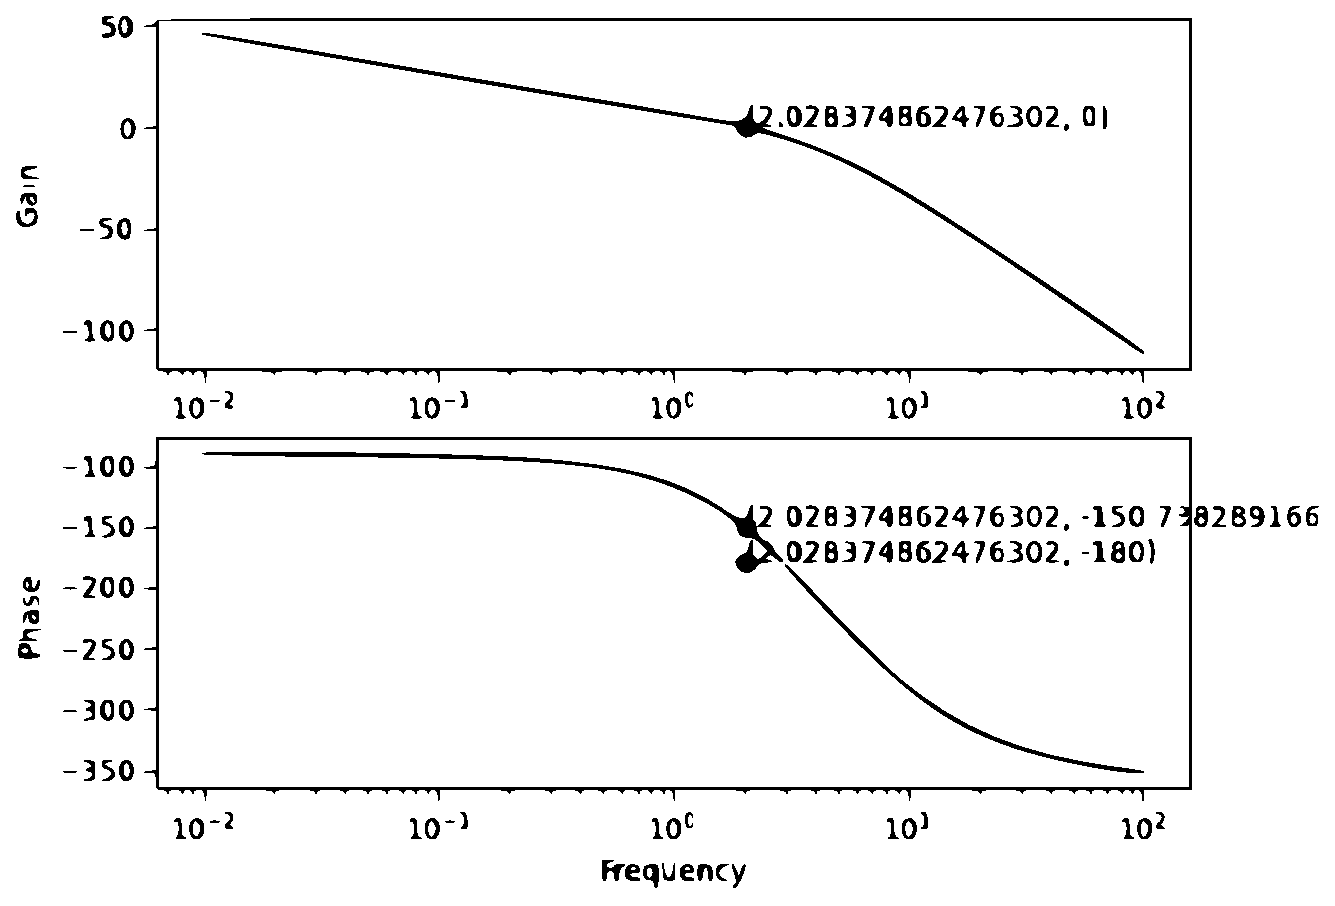
\includegraphics[width=\columnwidth]{./figs/es17btech11019_2.eps}
  \caption{}
  \label{fig:es17btech11019_2}
\end{figure}

Now for lag compensator of this whole lead compensated part
Transfer function:
\begin{align}
C'(s)=\brak{\frac{1+j\tau\omega}{1+j\alpha\tau\omega}}
\label{eq:es17btech11019_lag_compensator}
\end{align}

Find the values of $\alpha$ \\
\solution 

\begin{align}
\alpha=\frac{1}{\beta}
\label{eq:es17btech11019_alpha}
\end{align}

Solving equations \ref{eq:es17btech11019_alpha}
\begin{align}

\alpha=3.03
\label{eq:es17btech11019_final}
\end{align}

New Transfer Function:
\begin{align}
G(s)=\frac{96\brak{1+ 0.828s}\brak{1+0.828s}}{\brak{s}\brak{2+s}\brak{4+s}\brak{6+s}\brak{1+0.273s}\brak{1+2.50884s}}
\end{align}

Final plot is,

Find the plot using the following code
\begin{lstlisting}
codes/es17btech11019_4.py
\end{lstlisting}

\begin{figure}[!ht]
  \centering
  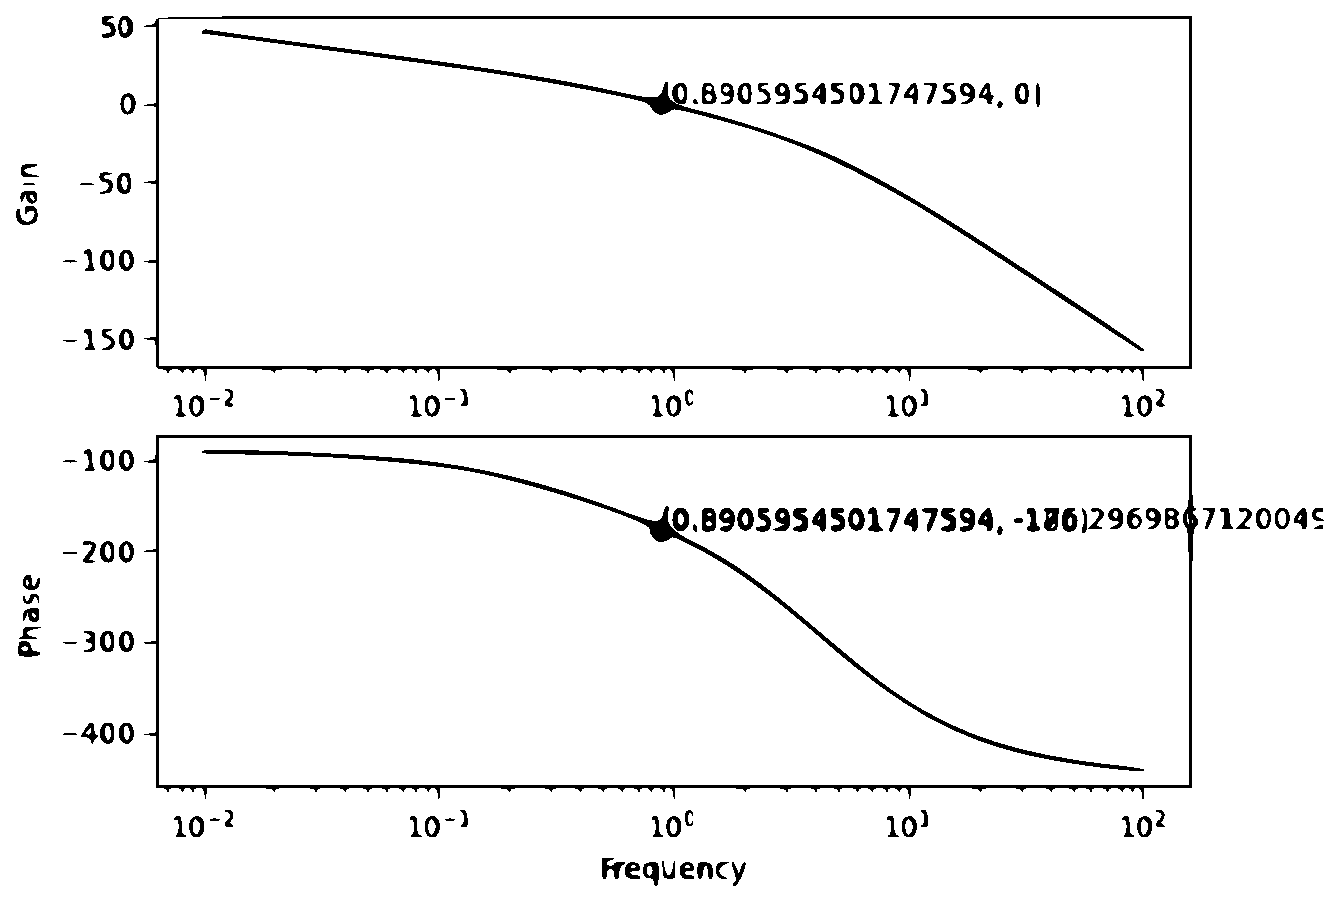
\includegraphics[width=\columnwidth]{./figs/es17btech11019_5}
  \caption{}
  \label{fig:es17btech11019_4}
\end{figure}


\end{enumerate}